\documentclass[11pt]{article}

\usepackage{amsmath, amsfonts, mathrsfs}
\usepackage{graphicx}
\usepackage{hyperref}
\hypersetup{
    colorlinks=true,
    linkcolor=blue,
    filecolor=magenta,      
    urlcolor=cyan
    }
\usepackage{tikz}
\usetikzlibrary{topaths,calc,hobby}

\usepackage[margin=0.97in,top=3cm,bottom=2cm, textheight=22.51cm,textwidth=16.51cm, heightrounded,columnsep=0.81cm]{geometry}

\newtheorem{theorem}{Theorem}
\newtheorem{corollary}[theorem]{Corollary}
\newtheorem{proposition}[theorem]{Proposition}
\newtheorem{lemma}[theorem]{Lemma}
\newtheorem{conjecture}[theorem]{Conjecture}
\newtheorem{problem}[theorem]{Problem}
\newtheorem{definition}[theorem]{Definition}
\newtheorem{example}[theorem]{Example}
\newtheorem{remark}[theorem]{Remark}

\title{Learning in Dynamic Matching Models}
\author{Shu Li \\
        Supervisor:  Ana Bu\v{s}i\'{c}, Jean-Michel Fourneau\\
        INRIA and ENS, PSL University}
\date{}

\begin{document}

\maketitle
%\tableofcontents
\section{Introduction}\label{sec:intro}

Stochastic matching models describe systems in which items of different classes arrive over time and depart only when matched with an item from a compatible class. A compatibility graph $G=(V,E)$ specifies feasible matches. We study the first-come--first-matched ({\textsc{FCFM}) discipline: upon arrival, if a compatible item is available in the buffer, the arriving item is matched with the earliest such item and the matched pair departs immediately; otherwise, the item is stored in the buffer. Throughout we normalize arrival rates so that $\mu(V)=\sum_{i\in V}\mu_i=1$ and adopt the convention that subscripts refer to singletons (e.g., $\mu_i,\Gamma_i$) while parentheses refer to sets (e.g., $\mu(S),\Gamma(S)$). Two structural results underpin our analysis: a necessary stability condition (\textsc{NCOND}) expressed via independent sets~\cite{MaMo18}, and a product-form stationary distribution for the buffer-content chain under \textsc{FCFM} on connected, non-bipartite graphs~\cite{MBMa21}. Formal notation and these facts are recalled in Section~\ref{sec:prelim}.

We first formalize the paradox in the baseline setting of simple graphs with unit weights.
Throughout this comparison, $G'$ denotes the graph obtained from $G$ by adding an edge (or, in the multigraph setting, a self-loop), and both models run under FCFM with the same arrival vector $\mu$ (normalized by $\mu(V)=1$).
We say that a performance paradox occurs when
\[
\mathbb{E}[G',\mu]>\mathbb{E}[G,\mu],
\]
i.e., the more compatible graph has a larger stationary total backlog. Sections~\ref{sec:matchcost} and~\ref{sec:abandon} extend this comparison to cost-weighted objectives $\mathbb{E}[G,\mu,c]$ and to models with abandonment $\mathbb{E}[G,\mu,\delta]$.

This report brings together three lines of work, all under \textsc{FCFM}. 
First, in the baseline setting of simple graphs with unit weights, we quantify how often paradoxes occur beyond isolated examples; to broaden coverage, we use an expected-value representation that also applies to multigraphs, showing that the effect appears across a range of graph families. 
Second, building on this baseline, we extend the comparison to the cost functional $\mathbb{E}[G,\mu,c]$ (notation fixed in Section~\ref{sec:prelim}) and derive closed-form evaluations on two benchmark graphs, the complete graph $K_n$ and the edge-deleted graph $K_n-\{1,2\}$ (Section~\ref{sec:matchcost}); for $K_n-\{1,2\}$ a refined normalizing constant isolates the two-step contribution of the independent set $\{1,2\}$. These formulas enable exact evaluation and a structured exploration of cost-weighted paradox regions. 
Third, we consider models with abandonment: although an exact product form is no longer directly available, a phase-error approximation allows us to evaluate the same comparison when items may leave before matching.

Product-form stationary distributions link redundancy systems and stochastic matching and provide a powerful starting point; yet obtaining performance metrics still requires aggregating a combinatorially large state space. The contributions above use product-form structure where available to produce explicit expected-value formulas and, when exact analysis is out of reach (with abandonment), deploy an approximation tailored to the matching dynamics. A broader synthesis of results on product forms, stability, greedy-policy paradoxes, cost-aware control, reneging, and graph generalizations is deferred to Section~\ref{sec:related}, after the model details.

Section~\ref{sec:prelim} sets notation and recalls \textsc{NCOND} and the product-form stationary distribution. Section~\ref{sec:related} reviews related work. Section~\ref{sec:partI} develops the multigraph expected-value expression and documents the prevalence of paradoxes across graph families. Section~\ref{sec:matchcost} formalizes the cost objective and presents closed-form evaluations on $K_n$ (Section~\ref{subsec:Kn}) and $K_n-\{1,2\}$ (Section~\ref{subsec:Kn12}), including the refined empty-state probability. Section~\ref{sec:abandon} treats abandonment via a phase-error approximation. Section~\ref{sec:comp-maps} reports computational evidence and paradox maps, and Section~\ref{sec:conclusions} concludes with design implications and directions for further work.

\section{Preliminaries}\label{sec:prelim}

We begin with a finite, simple, undirected compatibility graph $G=(V,E)$ with $|V|=n$ and no self-loops.
Items of class $i\in V$ arrive i.i.d.\ with class distribution $\mu=(\mu_i)_{i\in V}$; throughout we normalize $\mu(V)=\sum_{i\in V}\mu_i=1$.
Matching is performed under \textsc{FCFM}: upon arrival, if a compatible item is available in the buffer, the arriving item is matched with the earliest such item and the matched pair departs immediately; otherwise, the item is stored in the buffer.

Singletons use subscripts; sets use parentheses. For $i\in V$ and $S\subseteq V$,
\[
\mu_i:=\mu(\{i\}),\qquad 
\Gamma_i:=\{\,j\in V:\{i,j\}\in E\,\},\qquad
\mu(S):=\sum_{i\in S}\mu_i,\qquad 
\Gamma(S):=\bigcup_{i\in S}\Gamma_i.
\]
When unambiguous we identify a singleton with its element and use $\mu(\Gamma_i)$ as shorthand for $\mu(\Gamma(\{i\}))$.

Buffer content is represented by a \emph{word} $w=(w(1),\ldots,w(\ell(w)))$ over $V$ listed in order of arrival; write $|w|_i$ for the number of occurrences of $i$ in $w$.
A word $w$ is \emph{admissible} if no two letters in $w$ are adjacent in $G$; equivalently, the set of distinct letters in $w$ is an independent set of $G$.
Let $W$ denote the (countable) set of admissible words, including $\emptyset$, and let $\mathcal{I}$ be the family of nonempty independent sets of $G$.

A necessary condition for positive recurrence of the \textsc{FCFM} buffer-content chain is
\begin{equation}\label{eq:ncond}
\mu(I)<\mu\bigl(\Gamma(I)\bigr)\qquad\text{for every } I\in\mathcal{I}. 
\end{equation}
In particular, if $G$ is bipartite with bipartition $(A,B)$ then applying \eqref{eq:ncond} to $I=A$ and to $I=B$ yields a contradiction; hence such graphs cannot be positive recurrent under \textsc{FCFM}.
Throughout, statements under stationarity presuppose positive recurrence (e.g., \textsc{NCOND} holds).

On connected, non-bipartite simple graphs, the \textsc{FCFM} buffer-content chain admits a product-form stationary distribution.
For $w=(w(1),\ldots,w(\ell(w)))\in W$,
\begin{equation}\label{eq:product-form}
\pi(w)=\pi_{\emptyset}\prod_{k=1}^{\ell(w)}
\frac{\mu_{w(k)}}{\mu\bigl(\Gamma(\{w(1),\ldots,w(k)\})\bigr)},
\end{equation}
where the normalizing constant $\pi_{\emptyset}$ (the empty-state probability) is
\begin{equation}\label{eq:pi0-general}
\pi_{\emptyset}^{-1}=1+\sum_{I\in\mathcal{I}}\sum_{\sigma\in \mathfrak{S}_{|I|}}\prod_{k=1}^{|I|}
\frac{\mu_{i_{\sigma(k)}}}{\mu\bigl(\Gamma(\{i_{\sigma(1)},\ldots,i_{\sigma(k)}\})\bigr)-\mu\bigl(\{i_{\sigma(1)},\ldots,i_{\sigma(k)}\}\bigr)},
\end{equation}
with $I=\{i_1,\ldots,i_{|I|}\}$ and $\mathfrak{S}_{|I|}$ the permutation group on $|I|$ elements.

Assuming positive recurrence, let $W_\infty$ be a random word with law $\pi(\cdot)$ on $W$, i.e., $\mathbb{P}\{W_\infty=w\}=\pi(w)$ for all $w\in W$.
For $i\in V$,
\begin{equation}\label{eq:defqi}
Q_i:=|W_\infty|_i,\qquad 
\mathbb{E}[Q_i]=\sum_{w\in W}\pi(w)|w|_i.   
\end{equation}
For a graph $G$ and arrival vector $\mu$ with $\mu(V)=1$, define
\begin{equation}\label{eq:expqi}
\mathbb{E}[G,\mu]:=\sum_{i\in V}\mathbb{E}[Q_i]
\end{equation}
For the cost vector $c$, we define 
\begin{equation}\label{eq:expcqi}
\mathbb{E}[G,\mu,c]:=\sum_{i\in V}c_i\,\mathbb{E}[Q_i].   
\end{equation}
When abandonment $\delta$ is present
\begin{equation}\label{eq:expdqi}
\mathbb{E}[G,\mu,\delta]:=\sum_{i\in V}\mathbb{E}\left[Q_i^{(\delta)}\right].    
\end{equation}
Later sections evaluate these functionals exactly via \eqref{eq:product-form}–\eqref{eq:pi0-general}.

When self-loops are allowed, we work with a multigraph $G=(V,E)$.
Let 
\[
V_1:=\{\,i\in V:\{i,i\}\in E\,\},\qquad V_2:=V\setminus V_1,
\]
and let $\check{G}=(V,\mathcal{E})$ be the loop-deleted simple graph, $\mathcal{E}=E\setminus\{\{i,i\}:i\in V_1\}$.
Neighborhoods $\Gamma_i$ and $\Gamma(S)$ are computed on $\check{G}$, and admissible words obey:
(i) for any $\{i,j\}\in \mathcal{E}$ with $i\ne j$, $|w|_i\,|w|_j=0$;
(ii) for any $i\in V_1$, $|w|_i\le 1$.
The product-form extends to connected, non-bipartite multigraphs as
\begin{equation}\label{eq:product-form-multi}
\pi(w)\;=\;\pi_{\emptyset}\;\prod_{k=1}^{\ell(w)}
\frac{\mu_{\,w(k)}}{\mu\!\bigl(\Gamma(\{w(1),\ldots,w(k)\})\bigr)\;-\;\mu\!\bigl(\{w(1),\ldots,w(k)\}\cap V_2\bigr)},
\end{equation}
with normalizer
\begin{equation}\label{eq:pi0-multi}
\pi_{\emptyset}^{-1}=1+\sum_{I\in\mathcal{I}}\sum_{\sigma\in \mathfrak{S}_{|I|}}\prod_{k=1}^{|I|}
\frac{\mu_{i_{\sigma(k)}}}{\mu\bigl(\Gamma(\{i_{\sigma(1)},\ldots,i_{\sigma(k)}\})\bigr)-\mu\bigl(\{i_{\sigma(1)},\ldots,i_{\sigma(k)}\}\cap V_2\bigr)}.
\end{equation}
The simple-graph case is recovered when $V_1=\emptyset$, in which \eqref{eq:product-form-multi}–\eqref{eq:pi0-multi} reduce to \eqref{eq:product-form}–\eqref{eq:pi0-general}.

Two simple graphs will be analyzed in closed form: the complete graph $K_n$ and the edge-deleted graph $K_n-\{1,2\}$.
For both, $V_1=\emptyset$, so \eqref{eq:product-form}–\eqref{eq:pi0-general} apply.
In $K_n-\{1,2\}$ we will use $\Gamma_1=\Gamma_2=\{3,\dots,n\}$, hence $\mu(\Gamma_1)=\mu(\Gamma_2)=\mu(\Gamma(\{1,2\}))$.

\section{Related Work}\label{sec:related}

Recent surveys and research on product-form stationary distributions highlight connections between redundancy systems and stochastic matching, and document cases where such structures extend across modeling variants. A recurring theme is that having a product form does not by itself yield performance metrics: evaluating expectations typically requires aggregating a combinatorially large state space. Our report uses these structural results as a starting point to obtain explicit expected-value formulas and closed-form evaluations on selected graphs, which will be used for the paradox comparisons developed later.

For the stochastic matching model, the necessary stability condition (\textsc{NCOND}) is expressed via independent sets \cite{MaMo18}. Under \textsc{FCFM}, the buffer-content chain on connected, non-bipartite graphs admits a product-form stationary distribution; this has been established for simple graphs and extended to multigraphs (allowing self-loops), with explicit normalizing constants built from independent-set expansions \cite{MBMa21,BMMR20}. These results provide the structural basis used throughout our analysis.

A line of work documents that greedy matching may be non-monotone with respect to compatibility: adding edges or increasing flexibility can degrade stationary performance. Recent papers develop such “flexibility can hurt’’ effects under various objectives and graph structures, offering structural explanations tied to bottlenecks and independent sets \cite{BCDF24,CDFB21}. Our contributions align with this theme by giving exact evaluations (and, with abandonment, approximations) that expose where and why paradoxes arise.

Beyond fixed-policy evaluation, there is a substantial literature on optimizing objectives that include holding costs. Examples include finite-horizon holding-cost minimization in models close to matching, pricing-based control of arrival rates in assemble-to-order systems with queueing costs and expedite terms (via discrete-review policies), stabilizability and throughput optimality, and long-run average holding-cost minimization on bipartite systems \cite{gurvich2014,BGMa13,nazari2019}. In contrast, our cost-based study works under \textsc{FCFM} and provides exact closed forms (or approximations with abandonment) rather than proposing a control policy.

When items may abandon before matching, exact product forms are generally unavailable; analysis often proceeds via approximations or asymptotics. We adopt a phase-error approximation tailored to \textsc{FCFM} dynamics to show that performance paradoxes persist with abandonment, highlighting robustness of the phenomenon beyond the exact product-form setting.

Generalizing from simple graphs to multigraphs introduces self-loop classes and modifies admissible states and normalizing constants via independent-set sums over the loop-free projection. We provide an explicit expected-value expression on multigraphs, extending known formulas from simple graphs; on the simple-graph side, we derive closed forms for $K_n$ and $K_n-\{1,2\}$ and use them to map paradox regions under cost. Together these results complement prior structural insights by supplying computable formulas and reproducible evidence across objectives and modeling features.

\section{Performance paradoxes are not that rare}\label{sec:partI}
We compare graphs on the same vertex set $(V,\mu)$ under the same policy and say a paradox occurs if the evaluation on $G'$—obtained from $G$ by adding an edge (or a self-loop in the multigraph case)—exceeds that on $G$.
We work throughout under \textsc{FCFM} with arrivals $\mu=(\mu_i)_{i\in V}$ normalized by $\mu(V)=1$, and we use the multigraph notation of Section~\ref{sec:prelim}: self-loop classes $V_1$, loop-free classes $V_2=V\setminus V_1$, loop-deleted graph $\check{G}=(V,\mathcal{E})$, neighborhoods $\Gamma_i$ and $\Gamma(S)$ defined on $\check{G}$, and admissible words $W$. The necessary stability condition (\textsc{NCOND}) and the product-form stationary distribution with normalizing constant $\pi_{\emptyset}$ are recalled in \eqref{eq:ncond}–\eqref{eq:pi0-multi}.

We now rewrite the sum over all words $w$ as a finite sum over independent sets of $\check{G}$. 
For $\mathcal{I}\in\mathbb{I}(\check G)$,  fix an arbitrary ordering 
$\mathcal{I}^o=\{e_1,\dots,e_{|\mathcal{I}|}\}$. Given a permutation $\sigma$ 
of the index set $\{1,\dots,|\mathcal{I}|\}$, define the reordered 
list $\mathcal{I}^{\sigma(o)}=\{e_{\sigma(1)},\dots,e_{\sigma(|\mathcal{I}|)}\},$
that is, the sequence obtained by applying 
$\sigma$ to the ordered version $\mathcal{I}^o$. 
 We denote $\mathcal{I}_k^o$ as the first $k$ elements of $\mathcal{I}^o$.
Let $\mathcal{J}_k^o=\mathcal{I}_k^o\cap \mathcal{V}_2$. 
We define 
\begin{equation}
T_{\mathcal{I}^o}=\prod_{k=1}^{|\mathcal{I}|}\frac{\mu(\{e_{k}\})}{\mu\Bigl(\Gamma\bigl(\mathcal{I}_k^o\bigr)\Bigr)-\mu\Bigl(\mathcal{J}_k^o\Bigr)},
\end{equation}
and $T_{\mathcal{I}}=\sum_{\sigma \in \mathfrak{S}_{|\mathcal{I}|}} T_{\mathcal{I}^{\sigma(o)}}$. Thus $\pi(\emptyset) = (1 +T_{\mathcal{I}})^{-1}$. 
We also define
\begin{equation}
E_{\mathcal{I}^o}=\sum_{l=1}^{|\mathcal{I}|}
\frac{\mu\Bigl(\Gamma\bigl(\mathcal{I}_l^o\bigr)\Bigr)}
{\mu\Bigl(\Gamma\bigl(\mathcal{I}_l^o\bigr)\Bigr)-
\mu\Bigl(\mathcal{J}_l^o\Bigr)}\prod_{k=1}^{|\mathcal{I}|}
\frac{\mu(\{e_{k}\})}{\mu\Bigl(\Gamma\bigl(\mathcal{I}_k^o\bigr)\Bigr)-
\mu\Bigl(\mathcal{J}_k^o\Bigr)},   
\end{equation}
and $E_{\mathcal{I}}=\sum_{\sigma \in \mathfrak{S}_{|\mathcal{I}|}} E_{\mathcal{I}^{\sigma(o)}}$.

\begin{theorem}
[Expectation]\label{cor:exp-multi}
The expected number of items in steady state is
\begin{equation}\label{eq:exp-multi}
\mathbb{E}[G,\mu]=\Bigl(1+\sum_{\mathcal{I}\in\mathbb{I}(\check G)}T_\mathcal{I}\Bigr)^{-1}\sum_{\mathcal{I}\in\mathbb{I}(\check G)}E_\mathcal{I}.
\end{equation}
\end{theorem}

\begin{remark}
If $V_1=\emptyset$ ($V_2=\emptyset$), then Equation~\eqref{eq:exp-multi} reduces to product form of simple graph (full self-loop graph, respectively).
\end{remark}
We compare graphs on the same vertex set $(V,\mu)$ under the same policy and write $G'$ for the graph obtained from $G$ by adding an edge (or, in the multigraph setting, a self-loop). We declare a paradox when
\[
\mathbb{E}[G',\mu]>\mathbb{E}[G,\mu],
\]
that is, when the stationary total backlog $\sum_{i\in V}\mathbb{E}[Q_i]$—evaluated via \eqref{eq:exp-multi}—is larger on $G'$ than on $G$. Using \eqref{eq:ncond} to filter feasible $\mu$ and the explicit representation \eqref{eq:exp-multi}, we find that across a range of graph families (including multigraphs with self-loops and their simple-graph counterparts) there are sizable regions of $\mu$ where adding an edge increases the stationary. In our simulation, paradoxes concentrate near bottlenecks indicated by independent sets $I\in\mathcal{I}$ with $\mu(I)$ close to $\mu(\Gamma(I))$, consistent with the denominators $d_k$ that govern \eqref{eq:exp-multi}. This structural picture will reappear in later closed-form evaluations and in the empirical maps reported in Section~\ref{sec:comp-maps}.

The representation \eqref{eq:exp-multi} is explicit once independent sets of $\check{G}$ are available. For moderate $|V|$ and sparse graphs, enumerating $\mathcal{I}$ and evaluating the nested denominators $d_k$ is practical; for denser graphs, sampling orders $\sigma$ and pruning by \textsc{NCOND} provide scalable approximations. In Section~\ref{sec:paradox} we adopt a common Monte Carlo protocol (Dirichlet draws for $\mu$ with $\mu(V)=1$, \textsc{NCOND} checks on both graphs) to map paradox regions; exact closed forms for $K_n$ and $K_n-\{1,2\}$ then serve as controllable test cases for the same phenomenon under heterogeneous costs.

In what follows we compare graphs on a common $(V,\mu)$ under \textsc{FCFM} and say a paradox occurs if the left-hand side of \eqref{eq:exp-multi} when $V_1=\emptyset$ is larger on the more compatible graph. We summarize representative findings here; the sampling scheme—random draws of $\mu$ on the simplex with $\mu(V)=1$, \textsc{NCOND} screening, and graph-family generation—together with methodological details and extended figures is deferred to Section~\ref{sec:comp-maps}.

\section{Performance paradox in matching models with cost}\label{sec:matchcost}

Given class-dependent holding-cost rates $c=(c_i)_{i\in V}$ with $c_i>0$, we evaluate performance under \textsc{FCFM} via the stationary expected total holding cost
\begin{equation}\label{eq:def-cost}
E[G,\mu,c]:=\sum_{i\in V} c_i\mathbb{E}[Q_i],
\end{equation}
where $Q_i$ is defined in \eqref{eq:defqi} and expectations are taken with respect to the product-form stationary distribution when the chain is positive recurrent.

%\subsection{Complete graph $K_n$}\label{subsec:Kn}
On $K_n$ any two distinct classes are compatible. By \eqref{eq:product-form}–\eqref{eq:pi0-general}, only single-letter words are admissible; hence class-$i$ backlogs are geometric.

\begin{proposition}[Closed form on $K_n$]\label{prop:Kn}
Assume \textsc{NCOND} (equivalently $\mu_i<\mu(\Gamma_i)=\sum_{j\neq i}\mu_j$ for all $i$).
Then
\begin{equation}\label{eq:KnCost}
E[K_n,\mu,c]=\pi_{\emptyset}\sum_{i=1}^n\frac{c_i\,\mu(\Gamma_i)\,\mu_i}{\bigl(\mu(\Gamma_i)-\mu_i\bigr)^2},
\qquad
\pi_{\emptyset}
=\Bigl(1+\sum_{i=1}^n \frac{\mu_i}{\mu(\Gamma_i)-\mu_i}\Bigr)^{-1}.
\end{equation}
\end{proposition}

%\subsection{Edge-deleted graph $K_n-\{1,2\}$}\label{subsec:Kn12}
On $K_n-\{1,2\}$, here $\Gamma_1=\Gamma_2=\{3,\dots,n\}$ so that $\mu(\Gamma_1)=\mu(\Gamma_2)=\mu(\Gamma(\{1,2\}))$; classes $1$ and $2$ cannot match each other and may coexist.

\begin{proposition}[Closed form on $K_n-\{1,2\}$]\label{prop:Kn12}
Assume \textsc{NCOND}. Then
\begin{equation}\label{eq:KnMinusCost}
E[K_n-\{1,2\},\mu,c]
\;=\;
\pi_{\emptyset}\Biggl(
\sum_{i=3}^n \frac{c_i\,\mu(\Gamma_i)\,\mu_i}{\bigl(\mu(\Gamma_i)-\mu_i\bigr)^2}+\frac{\mu(\Gamma_1)\,\bigl(c_1\mu_1+c_2\mu_2\bigr)}
{\bigl(\mu(\Gamma_1)-\mu_1-\mu_2\bigr)^2}
\Biggr),
\end{equation}
with
\begin{equation}\label{eq:pi0KnMinus}
\pi_{\emptyset}
=\Biggl(1+\sum_{i=1}^n \frac{\mu_i}{\mu(\Gamma_i)-\mu_i}
+\frac{\mu_1\mu_2}{(\mu(\Gamma_1)-\mu_1)(\mu(\Gamma_1)-\mu_1-\mu_2)}
+\frac{\mu_1\mu_2}{(\mu(\Gamma_1)-\mu_2)(\mu(\Gamma_1)-\mu_1-\mu_2)}\Biggr)^{-1}.
\end{equation}
\end{proposition}

\paragraph{Use in paradox comparisons.}
Formulas \eqref{eq:KnCost}–\eqref{eq:KnMinusCost} enable direct cost comparisons on $K_n$ vs.\ $K_n-\{1,2\}$ under the same $(\mu,c)$ and $\mu(V)=1$. In Section~\ref{sec:comp-maps} we report parameter regions where $E[K_5,\mu,c]>E[K_5-\{1,2\},\mu,c]$ (or the reverse), and in Section~\ref{sec:comp-maps} we describe the common sampling and verification protocol used to generate these regions.

\section{Performance paradox in matching models with abandonment}\label{sec:abandon}

Matching models with abandonment have not yet been solved for any compatibility graph. 
Therefore, we restrict ourselves to two very simple compatibility graphs: the complete graph $K_n$ and $K_n - (1,2)$, the same graph where we have removed edge $(1,2)$. 
These graphs are so simple that we can find the steady-state distributions for the associated Markov chains and study the 
ergodicity of the chains. 
Note have also used these two graphs in \cite{CDFB21} to prove the performance paradox on matching model without abandonment. 

\emph{Complete graph \(K_n\).} The steady-state probability for being in state $(i,m)$ is given by:
\begin{equation}
\pi_{i,m} = \pi_0\prod_{k=1}^{m} \frac{\mu_i}{\mu(\Gamma_i) + k \delta} \quad \text{for } i=1, 2, \dots, n.
\end{equation}
The expected total population in the system, denoted by $\mathbb{E}[N_1 + N_2 + \cdots + N_n]$, is the sum of the expected number of individuals in each class. 
This can be expressed as:
\begin{equation}
\mathbb{E}[N_1 + N_2 + \cdots + N_n] = \sum_{i=1}^{n} \sum_{m=1}^{\infty} m \pi_{i,m}.
\end{equation}
Substituting the expression for $\pi_{i,m}$:
\begin{equation}
\mathbb{E}[K_n, \mu] = \sum_{i=1}^{n} \sum_{m=1}^{\infty} m~ \pi_0\prod_{k=1}^{m} \frac{\mu_i}{\mu(\Gamma_i) + k \delta}.
\end{equation}
This provides the expected number of individuals in the system by summing over the states of all classes, weighted by the steady-state probabilities.

Let \(G=K_n-\{1,2\}\) and define an aggregation that identifies classes \(1\) and \(2\) into a single class \(a\).
By strong lumpability for continuous-time Markov chains \cite{BaYe93}, the \textsc{FCFM} buffer-content chain on \(G\) is lumpable with respect to the partition that merges letters \(1\) and \(2\).
The lumped chain is exactly the \textsc{FCFM} chain on the complete graph with \(n-1\) classes,
\[
K_{n-1}\ \text{ on the class set }\ \{a,3,4,\dots,n\},
\]
with parameters obtained by aggregation:
\[
\mu'_a=\mu_1+\mu_2,\quad \mu'_j=\mu_j\ (j\ge3),\quad \delta'=\delta
\]
and neighborhoods
\[
\Gamma'_a=\{3,\dots,n\},\quad \Gamma'_j=\{a,3,\dots,n\}\setminus\{j\},\qquad
\mu(\Gamma'_a)=\mu\!\bigl(\Gamma(\{1,2\})\bigr).
\]
Consequently, the total (unweighted) stationary backlog with abandonment satisfies the reduction
\begin{equation}\label{eq:lump-Kn12}
\mathbb{E}[K_n-\{1,2\},\mu,\delta]=\mathbb{E}[K_{n-1},\mu',\delta'],
\end{equation}
where the right-hand side is evaluated by the \(K_{n-1}\) closed form in \eqref{eq:Kn-PEA} with \((\mu',\delta')\) in place of \((\mu,\delta)\).
Equivalently, the empty-state probability obeys the same aggregation:
\begin{equation}\label{eq:lump-pi0}
\pi_{\emptyset}^{(\delta)}(K_n-\{1,2\},\mu,\delta)=
\pi_{\emptyset}^{(\delta)}(K_{n-1},\mu',\delta')=\Biggl(1+\sum_{i\in\{a,3,\dots,n\}}\frac{\mu'_i}{\mu(\Gamma'_i)+\delta'-\mu'_i}\Biggr)^{-1}.
\end{equation}

\noindent\emph{Rationale.}
On \(K_n-\{1,2\}\) we have \(\Gamma_1=\Gamma_2=\{3,\dots,n\}\) and there is no \(1\)–\(2\) edge; under \textsc{FCFM}, arrivals of class \(1\) or \(2\) are indistinguishable to all other classes and to each other except for their labels.
The transition rates of the detailed chain depend on \(1\) and \(2\) only through the sums \(\mu_1+\mu_2\) and \(\delta_1+\delta_2\), and through the shared neighborhood \(\Gamma(\{1,2\})\).
Therefore, for any two detailed states that differ only by permuting \(1\) and \(2\), the aggregated exit rates to each block are equal, satisfying the strong lumpability conditions; the lumped dynamics coincide with \textsc{FCFM} on \(K_{n-1}\) with the aggregated parameters above.

\section{Computational framework and examples}\label{sec:comp-maps}

We consolidate the implementation details and empirical results into a single section. 
All scripts, configuration files, and notebooks needed to reproduce the figures and tables below are publicly available; see the repositories \cite{li2025,li2025a,li2025b}.

\begin{figure}[htbp]
\centering
\begin{minipage}{0.4\textwidth}
\centering
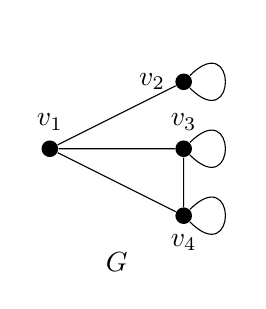
\begin{tikzpicture}[scale=0.85, vertex/.style={minimum width=6pt, circle, inner sep=0pt}]
\node at (0,-1.7){$G$};
\node[vertex,fill,label=above:$v_1$] (1) at (-1,0) {};
\node[vertex,fill,label=left:$v_2$] (2) at (1,1) {};
\node[vertex,fill,label=above:$v_3$] (3) at (1,0) {};
\node[vertex,fill,label=below:$v_4$] (4) at (1,-1) {};
\draw (2) to [out=45, in=315, loop, min distance=1cm](2);
\draw (3) to [out=45, in=315, loop, min distance=1cm](3);
\draw (4) to [out=45, in=315, loop, min distance=1cm](4);
\draw (2)--(1)--(3)--(4)--(1);
\end{tikzpicture}
\end{minipage}
\hspace{2pt}
\begin{minipage}{0.4\textwidth}
\centering
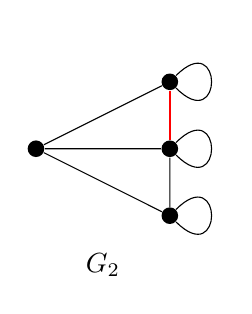
\begin{tikzpicture}[scale=0.85, vertex/.style={minimum width=6pt, circle, inner sep=0pt}]
\node at (0,-1.74){$G_2$};
\node[vertex,fill] (1) at (-1,0) {};
\node[vertex,fill] (2) at (1,1) {};
\node[vertex,fill] (3) at (1,0) {};
\node[vertex,fill] (4) at (1,-1) {};
\draw (2) to [out=45, in=315, loop, min distance=1cm](2);
\draw (3) to [out=45, in=315, loop, min distance=1cm](3);
\draw (4) to [out=45, in=315, loop, min distance=1cm](4);
\draw (2)--(1)--(3)--(4)--(1);
\draw[thick,red] (2)--(3);
\end{tikzpicture}
\end{minipage}
\caption{Graphs: $G$ and $G_2$.}
\label{fig:gandmc}
\end{figure}


\begin{figure}[hbtp]
\centering
\begin{minipage}{0.45\textwidth}
\centering
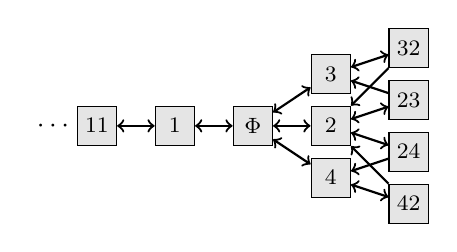
\begin{tikzpicture}[scale=0.66, state/.style={minimum width=5mm, minimum height=5mm, draw=black, fill=gray!20, inner sep=0pt, font=\footnotesize}]
\node[state] (0) at (0,0) {$\Phi$};
\node[state] (1) at (-1.5,0) {$1$};
\node[state] (11) at (-3,0) {$11$};
\node (111) at (-3.8,0) {$\cdots$};
\node[state] (3) at (1.5,1) {$3$};
\node[state] (2) at (1.5,0) {$2$};
\node[state] (4) at (1.5,-1) {$4$};
\node[state] (32) at (3,1.5) {$32$};
\node[state] (23) at (3,0.5) {$23$};
\node[state] (24) at (3,-0.5) {$24$};
\node[state] (42) at (3,-1.5) {$42$};

\draw[thick,<->](0)--(1);
\draw[thick,<->](11)--(1);
\draw[thick,<->](0)--(3);
\draw[thick,<->](0)--(2);
\draw[thick,<->](0)--(4);
\draw[thick,<->](3)--(32);
\draw[thick,<->](2)--(24);
\draw[thick,<->](2)--(23);
\draw[thick,<->](4)--(42);
\draw[thick,->](32)--(2);
\draw[thick,->](42)--(2);
\draw[thick,->](23)--(3);
\draw[thick,->](24)--(4);
\end{tikzpicture}
\end{minipage}
\vspace{2pt}
\begin{minipage}{0.45\textwidth}
\centering
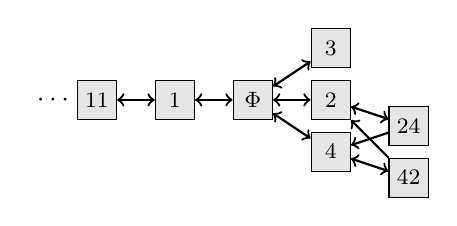
\begin{tikzpicture}[scale=0.66, state/.style={minimum width=5mm, minimum height=5mm, draw=black, fill=gray!20, inner sep=0pt, font=\footnotesize}]
\node[state] (0) at (0,0) {$\Phi$};
\node[state] (1) at (-1.5,0) {$1$};
\node[state] (11) at (-3,0) {$11$};
\node (111) at (-3.8,0) {$\cdots$};
\node[state] (3) at (1.5,1) {$3$};
\node[state] (2) at (1.5,0) {$2$};
\node[state] (4) at (1.5,-1) {$4$};
%\node[state] (32) at (3,1.5) {$32$};
%\node[state] (23) at (3,0.5) {$23$};
\node[state] (24) at (3,-0.5) {$24$};
\node[state] (42) at (3,-1.5) {$42$};

\draw[thick,<->](0)--(1);
\draw[thick,<->](11)--(1);
\draw[thick,<->](0)--(3);
\draw[thick,<->](0)--(2);
\draw[thick,<->](0)--(4);
%\draw[thick,<->](3)--(32);
\draw[thick,<->](2)--(24);
%\draw[thick,<->](2)--(23);
\draw[thick,<->](4)--(42);
%\draw[thick,red,->](32)--(2);
\draw[thick,->](42)--(2);
%\draw[thick,red,->](23)--(3);
\draw[thick,->](24)--(4);
\end{tikzpicture}
\end{minipage}
\caption{Truncation of the Markov Chains for $G$ (left) and  $G_2$ (right).}
\label{fig:mc}
\end{figure}

We consider $G=(\mathcal{V},\mathcal{E})$ in Fig.~\ref{fig:gandmc}, where $\mathcal{V}$ is partitioned into $\mathcal{V}_1=\{v_2, v_3, v_4\}$ and $\mathcal{V}_2=\{v_1\}$. The independent sets of $\check{G}$ are 
$
\{\{v_1\}, \{v_2\}, \{v_3\}, \{v_4\}, \{v_2,v_4\}, \\
\{v_2,v_3\}\}
$.
Graph $G_2$ is 
obtained by inserting the edge $\{v_2,v_3\}$ (see Fig.~\ref{fig:gandmc}). The associated Markov Chains, 
truncated to states with at most two letters, are depicted in Fig.~\ref{fig:mc}. 
The rates are 
$\lambda_1 = 0.432685$, 
$\lambda_2 = 0.005861$, $\lambda_3 = 0.141128$ and 
$\lambda_4 = 0.420326$. The bottleneck set is a singleton (i.e. $\{v_1\})$. 
We have a paradox as the expectation slightly increases from 
$2.944793$ to $2.947256$ when we add the edge. 
\begin{figure}[htbp]
\centering
\begin{minipage}{0.22\textwidth}
\centering
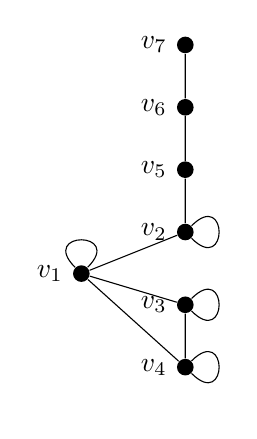
\begin{tikzpicture}[scale=0.66, vertex/.style={minimum width=6pt, circle, inner sep=0pt}]
\node[vertex,fill, label=left:$v_1$](1) at (-1,0){};
\node[vertex,fill, label=left:$v_2$](2) at (1,0.8){};
\node[vertex,fill, label=left:$v_3$](3) at (1,-0.6){};
\node[vertex,fill, label=left:$v_4$](4) at (1,-1.8){};
\node[vertex,fill, label=left:$v_5$](5) at (1,2){};
\node[vertex,fill, label=left:$v_6$](6) at (1,3.2){};
\node[vertex,fill, label=left:$v_7$](7) at (1,4.4){};
\draw (1) to [out=45, in=135, loop, min distance=1cm](1);
\draw (2) to [out=45, in=315, loop, min distance=1cm](2);
\draw (3) to [out=45, in=315, loop, min distance=1cm](3);
\draw (4) to [out=45, in=315, loop, min distance=1cm](4);
%\draw (5) to [out=45, in=315, loop, min distance=1cm](5);
\draw(1)--(3)--(4)--(1)--(2)--(5)--(6)--(7);
\end{tikzpicture}
\end{minipage}
\hspace{2pt}
\begin{minipage}{0.22\textwidth}
\centering
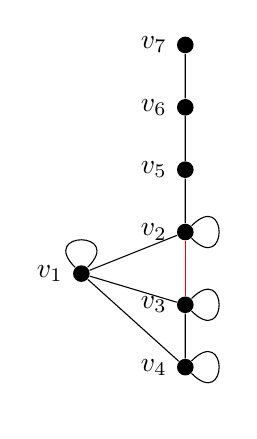
\begin{tikzpicture}[scale=0.66, vertex/.style={minimum width=6pt, circle, inner sep=0pt}]
\node[vertex,fill, label=left:$v_1$](1) at (-1,0){};
\node[vertex,fill, label=left:$v_2$](2) at (1,0.8){};
\node[vertex,fill, label=left:$v_3$](3) at (1,-0.6){};
\node[vertex,fill, label=left:$v_4$](4) at (1,-1.8){};
\node[vertex,fill, label=left:$v_5$](5) at (1,2){};
\node[vertex,fill, label=left:$v_6$](6) at (1,3.2){};
\node[vertex,fill, label=left:$v_7$](7) at (1,4.4){};
\draw (1) to [out=45, in=135, loop, min distance=1cm](1);
\draw (2) to [out=45, in=315, loop, min distance=1cm](2);
\draw (3) to [out=45, in=315, loop, min distance=1cm](3);
\draw (4) to [out=45, in=315, loop, min distance=1cm](4);
%\draw (5) to [out=45, in=315, loop, min distance=1cm](5);
\draw(1)--(3)--(4)--(1)--(2)--(5)--(6)--(7);
\draw[red] (2)--(3);
\end{tikzpicture}
\end{minipage}
\hspace{2pt}
\begin{minipage}{0.22\textwidth}
\centering
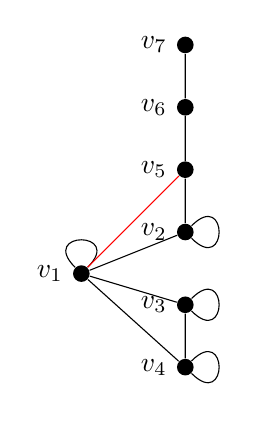
\begin{tikzpicture}[scale=0.66, vertex/.style={minimum width=6pt, circle, inner sep=0pt}]
\node[vertex,fill, label=left:$v_1$](1) at (-1,0){};
\node[vertex,fill, label=left:$v_2$](2) at (1,0.8){};
\node[vertex,fill, label=left:$v_3$](3) at (1,-0.6){};
\node[vertex,fill, label=left:$v_4$](4) at (1,-1.8){};
\node[vertex,fill, label=left:$v_5$](5) at (1,2){};
\node[vertex,fill, label=left:$v_6$](6) at (1,3.2){};
\node[vertex,fill, label=left:$v_7$](7) at (1,4.4){};
\draw (1) to [out=45, in=135, loop, min distance=1cm](1);
\draw (2) to [out=45, in=315, loop, min distance=1cm](2);
\draw (3) to [out=45, in=315, loop, min distance=1cm](3);
\draw (4) to [out=45, in=315, loop, min distance=1cm](4);
%\draw (5) to [out=45, in=315, loop, min distance=1cm](5);
\draw(1)--(3)--(4)--(1)--(2)--(5)--(6)--(7);
\draw[red](1)--(5);
\end{tikzpicture}
\end{minipage}
\hspace{2pt}
\begin{minipage}{0.22\textwidth}
\centering
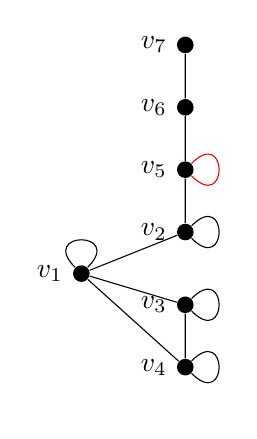
\begin{tikzpicture}[scale=0.66, vertex/.style={minimum width=6pt, circle, inner sep=0pt}]
\node[vertex,fill, label=left:$v_1$](1) at (-1,0){};
\node[vertex,fill, label=left:$v_2$](2) at (1,0.8){};
\node[vertex,fill, label=left:$v_3$](3) at (1,-0.6){};
\node[vertex,fill, label=left:$v_4$](4) at (1,-1.8){};
\node[vertex,fill, label=left:$v_5$](5) at (1,2){};
\node[vertex,fill, label=left:$v_6$](6) at (1,3.2){};
\node[vertex,fill, label=left:$v_7$](7) at (1,4.4){};
\draw (1) to [out=45, in=135, loop, min distance=1cm](1);
\draw (2) to [out=45, in=315, loop, min distance=1cm](2);
\draw (3) to [out=45, in=315, loop, min distance=1cm](3);
\draw (4) to [out=45, in=315, loop, min distance=1cm](4);
\draw[red] (5) to [out=45, in=315, loop, min distance=1cm](5);
\draw(1)--(3)--(4)--(1)--(2)--(5)--(6)--(7);
\end{tikzpicture}
\end{minipage}
\caption{graphs: $H$, $H_1$, $H_2$ and $H_3$. }
\label{fig:graphs_example2}
\end{figure}
The former example does not address the case of adding a new edge $e$ connecting a node lacking a self-loop to a node with self-loop. To fill this gap, we study graph $H_2$ (see Fig.\ref{fig:graphs_example2}),  obtained from $H$ by inserting edge $\{v_1,v_5\}$. Similarly, graph $H_1$ is formed by connecting $v_2$ and $v_3$, while graph $H_3$ is obtained by adding a self-loop to {$v_5$}. We have found performance paradoxes in all cases.
For arrival rate vector 
$( 0.070716, 0.180906, 0.238414, 0.204521,  0.164007, 0.07243, 
0.069006)$
the bottleneck set is $\{v_7\}$. The expectation is $31.218542$ for graph $H$ 
and it increases to 
$ 31.539906$ for graph $H_1$.  
Similarly, if we start with arrival rate vector 
$( 0.08502,  0.06418,  0.076071,  0.096493,  0.336406, 0.326572, 0.015258)$
for $H$, we get an expectation for the total number equal to $13.0179$ and the expectation is equal to $13.058815$ for the same rates and graph $H_2$. Finally, 
the comparison between $H$ and $H_3$ for rate vector $(0.104627, 0.052725,  0.194586, 0.190934, 0.117413, 0.225466,\\ 0.114249)$ also shows a performance
paradox: the expectation was $33.838547$ for $H$ and it jumps to $35.972599$ for $H_3$. In both cases, the bottleneck independent  set is singleton $\{v_6 \}$. 

\subsection{Paradox with cost for $K_5$ and $K_5-\{1,2\}$}
\begin{figure} [htbp]
\begin{center} 
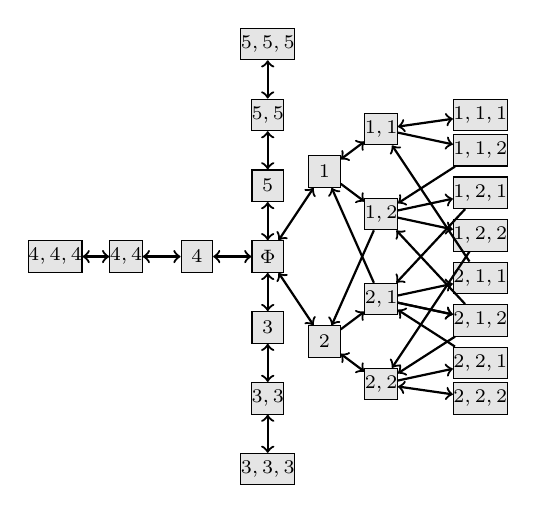
\begin{tikzpicture}[scale=0.9, state/.style={minimum width=4mm, minimum height=4mm, draw=black, fill=gray!20, inner sep=0pt, font=\scriptsize}]

\node[state] (0) at (0,0)  {$\Phi$};

\node[state] (5) at (0,1)  {$5$};
\node[state] (55) at (0,2)  {$5,5$};
\node[state] (555) at (0,3)  {$5,5,5$};

\node[state] (3) at (0,-1)  {$3$};
\node[state] (33) at (0,-2)  {$3,3$};
\node[state] (333) at (0,-3)  {$3,3,3$};

\node[state] (4) at (-1,0)  {$4$};
\node[state] (44) at (-2,0)  {$4,4$};
\node[state] (444) at (-3,0)  {$4,4,4$};

\draw[<->, thick] (444)--(44);
\draw[<->, thick] (333)--(33);
\draw[<->, thick] (555)--(55);

\foreach \x /\y in {44/4, 4/0, 55/5, 5/0, 0/3, 3/33}
{\draw[<->, thick] (\x)--(\y);}

\node[state] (1) at (0.8,1.2)  {$1$};
\node[state] (2) at (0.8,-1.2)  {$2$};

\node[state] (11) at (1.6,1.8)  {$1,1$};
\node[state] (12) at (1.6,0.6)  {$1,2$};
\node[state] (21) at (1.6,-0.6)  {$2,1$};
\node[state] (22) at (1.6,-1.8)  {$2,2$};

\draw[<->, thick] (0)--(1);
\draw[<->, thick] (0)--(2);

\draw[<->, thick] (1)--(11);
\draw[->, thick] (1)--(12);
\draw[->, thick] (21)--(1);
\draw[->, thick] (2)--(21);
\draw[<->, thick] (2)--(22);
\draw[->, thick] (12)--(2);

\node[state] (111) at (3,2.0)  {$1,1,1$};
\node[state] (112) at (3,1.5)  {$1,1,2$};
\node[state] (121) at (3,0.9)  {$1,2,1$};
\node[state] (122) at (3,0.3)  {$1,2,2$};
\node[state] (211) at (3,-0.3)  {$2,1,1$};
\node[state] (212) at (3,-0.9)  {$2,1,2$};
\node[state] (221) at (3,-1.5)  {$2,2,1$};
\node[state] (222) at (3,-2)  {$2,2,2$};

\foreach \a/\b in {11/111, 22/222} {
  \draw[<->, thick] (\a)--(\b);
}

\draw[->, thick] (11)--(112);
\draw[->, thick] (22)--(221);
\draw[->, thick] (21)--(212);

\foreach \a/\b in {11/211, 12/112, 21/121, 21/221, 22/122, 22/212, 12/212} {
  \draw[<-, thick] (\a)--(\b);
}

\foreach \a/\b in {12/121, 12/122, 21/211,21/212} {
  \draw[->, thick] (\a)--(\b);
}
\end{tikzpicture}
\end{center}
\caption{CTMC for $K_5=\{1,2\}$, restricted to states with less than $4$ items. \label{secondmodel}}
\end{figure}
With the arrival rates: $\mu_1=0.2123089053707668$, $\mu_2=0.2742714546697317$,
$\mu_3=0.006999635670957356$,
$\mu_4=0.009689658354828117$,
$\mu_5=0.4967303459337161$,
we consider the cost rates:
$c_1=2.7238918756873907$,
$c_2=2.4122427717406985$,
$c_3=0.7902759709551836$,
$c_4=1.6367962372371867$,
$c_5=2.941675109364959$. Our
algorithms provide $\mathbb{E}[K_5]=220.65202293442172$ and $\mathbb{E}[K_5-\{1,2\}]=190.10942991220702$.

With the arrival rates: $\mu_1=0.3636329852744427$, $\mu_2=0.12673427390852054$,
$\mu_3=0.010843072513621425$,
$\mu_4=0.00588355294263528$,
$\mu_5=0.4967303459337161$,
we consider the cost rates:
$c_1=0.7586371655061703$,
$c_2=0.5922847832917051$,
$c_3=1.2921580773128705$,
$c_4=1.5334451333796428$,
$c_5=2.7928617067309602$. Our
algorithms provide $\mathbb{E}[K_5]=93.13740159182518$ and $\mathbb{E}[K_5-\{1,2\}]=64.52734567817744$.

With the arrival rates: $\mu_1=0.3318483989009918$, $\mu_2=0.15555361051577288$,
$\mu_3=0.008889036408139615$,
$\mu_4=0.010680845648430016$,
$\mu_5=0.4930281085266657$,
we consider the cost rates:
$c_1=0.540035985717008$,
$c_2=0.7140147194846248$,
$c_3=2.4159213267991975$,
$c_4=0.9251339822272417$,
$c_5=2.019825022348815$. Our
algorithms provide $\mathbb{E}[K_5]=69.11018350819715$ and $\mathbb{E}[K_5-\{1,2\}]=50.80578875204731$.

With the arrival rates: $\mu_1=0.27213894636867086$, $\mu_2=0.2103851356861736$,
$\mu_3=0.021582541556846437$,
$\mu_4=0.00206614868091172$,
$\mu_5=0.4938272277073974$,
we consider the cost rates:
$c_1=2.0706759633272456$,
$c_2=1.0160689586750364$,
$c_3=2.32274822225199$,
$c_4=1.2423689869742887$,
$c_5=2.4547513725489267$. Our
algorithms provide $\mathbb{E}[K_5]=95.94786753522975$ and $\mathbb{E}[K_5-\{1,2\}]=79.43003650548351$.

\subsection{Paradox with Abandonment}
To demonstrate the performance paradox in the presence of abandonment, we present some numerical instances drawn 
from a large-scale Monte Carlo search. All results and programs 
are documented in~\cite{li2025a}. For all the examples 
presented in the following,
the truncation error $\epsilon$ is equal to $0.00001$ 
and the number of type of items (i.e. $n$) is $5$. 
Types 1 and 2 having equal arrival rates. For 
the sake of readability in the presentation of 
the results, we write $K_4$
instead of $K_5 - (1,2)$ as we have proved that the models are equivalent for the expectation. 

\paragraph{Abandonment rate $\delta=0.01$:}
we consider the following arrival rates:\\
$\mu_1=\mu_2=0.07198009646943532$, $\mu_3=0.1505252430731784$, \\
$\mu_4=0.2139285951521536$ and $\mu_5=0.49158596883579736$. 
Applying the certified truncation method, we obtain the two bounds for the expected total number of items as $\underline{\mathbb{E}}[K_5] = 4.517062201492523$ and 
$\overline{\mathbb{E}}[K_4] = 4.507590806996654$. Since $\underline{\mathbb{E}}[K_5] > \overline{\mathbb{E}}[K_4]$, this example certifies a paradox.

\paragraph{Abandonment rate $\delta=0.02$:}
With the arrival rates:
$\mu_1=\mu_2=0.137987656$,\\ $\mu_3=0.162773315$, 
$\mu_4=0.47490324$ and $\mu_5=0.086348129$
we get the following bounds: 
$\underline{\mathbb{E}}[K_5] = 2.705018525$ and 
$\overline{\mathbb{E}}[K_4] = 2.686966814$. Again a 
performance paradox.

\paragraph{Abandonment rate $\delta=0.05$:}
We consider the following arrival rates:
$\mu_1=\mu_2=0.070548153$, 
$\mu_3=0.248317959$, 
$\mu_4=0.116798768$ and $\mu_5=0.493786968$. We algorithms
provide the following bounds: 
$\underline{\mathbb{E}}[K_5] = 2.068573185$ and 
$\overline{\mathbb{E}}[K_4] = 2.066821283$. And we obtain a
new paradox: $\underline{\mathbb{E}}[K_5] > \overline{\mathbb{E}}[K_4]$.

\paragraph{Abandonment rate $\delta=0.07$:}
The following arrival rates:
$\mu_1=\mu_2=0.041846729$, $\mu_3=0.286078133$, 
$\mu_4=0.134189224$ and $\mu_5=0.496039185$
lead to 
$\underline{\mathbb{E}}[K_5] = 1.777650699$ and 
$\overline{\mathbb{E}}[K_4] = 1.777497359$. Again a performance
paradox as $\underline{\mathbb{E}}[K_5] > \overline{\mathbb{E}}[K_4]$.


\section{Conclusions and Future Work}\label{sec:conclusions}

This report assembles three complementary results on performance paradoxes for stochastic matching under \textsc{FCFM}. (i) At the structural level, we give an explicit expected-value representation on multigraphs, together with its specialization to simple graphs, and use it to show that paradoxes arise beyond isolated examples—across a range of graph families that satisfy \textsc{NCOND}. (ii) At the objective level, we obtain closed-form evaluations on the benchmark pair $K_n$ and $K_n-\{1,2\}$ for $\mathbb{E}[G,\mu,c]$, including a refined empty-state normalization on $K_n-\{1,2\}$; these formulas enable exact side-by-side comparisons under a common $(\mu,c)$ and reveal sizable cost-weighted paradox regions. (iii) At the modeling level, for systems with abandonment we develop a phase-error approximation and, via strong lumpability, reduce $K_n-\{1,2\}$ to $K_{n-1}$ by aggregating $\{1,2\}$; this yields tractable evaluators for $\mathbb{E}[G,\mu,\delta]$ on the same benchmarks. Two themes recur throughout: independent-set bottlenecks—made visible by the denominators in the product-form expansions—and the value of evaluable expressions that turn structural product forms into computable performance measures.

Looking ahead, several threads are natural. First, \emph{applications}: (a) cross-trained service systems and skill-based routing, where adding a few cross-compatibilities to a predominantly bipartite core (creating small odd-cycle augmentations) is common practice; our maps can inform whether a proposed compatibility edge is beneficial under given arrival mix; (b) substitution networks in assemble-to-order and inventory pooling, where partial substitutability induces compatibility graphs and the cost criterion $\mathbb{E}[G,\mu,c]$ is operationally meaningful; (c) redundancy-style computing and content delivery, which admit multigraph interpretations with self-loops and can be probed with the multigraph representation used here. Second, \emph{graph classes}: extend exact (or near-exact) evaluations beyond the two benchmarks to families that preserve tractable structure—e.g., $K_n$ minus a matching, $K_n$ minus a star, odd-cycle augmentations of bipartite cores, chordal and split graphs, and selected circulant or random graph models—seeking closed forms or controlled approximations. Third, \emph{design and policy}: formulate edge-addition/removal problems under $\mathbb{E}[G,\mu,c]$ as optimization tasks; examine sensitivity to tie-breaking and simple priority rules within \textsc{FCFM}; and refine the phase-error approximation by deriving error diagnostics or bounds and testing alternative patience embeddings. The computational artifacts for the present study (unweighted, cost-weighted, and abandonment settings) are released for reuse and extension; see \cite{li2025,li2025a,li2025b}.

\section{Academic Activities and Participation}\label{sec:activities}

This section summarizes my academic activities during the reporting period, including completion of the second-year report draft, research talks, conference participation, and editorial/reviewing service. The work disseminated in these venues consolidates three research threads under \textsc{FCFM}:

\begin{itemize}\itemsep0.25em
\item \emph{Performance paradoxes in matching systems are not that rare}(Sections~\ref{sec:partI}). NETGCOOP 2025, Accepted.
\item \emph{Performance paradox in matching models with cost}(Section~\ref{sec:matchcost}).
\item \emph{Performance paradox in matching models with abandonment}(Section~\ref{sec:abandon}). EAI VALUETOOLS 2025, Under review.
\end{itemize}
All code artifacts, configuration files, and scripts to reproduce the figures in Section~\ref{sec:comp-maps} are publicly released \cite{li2025,li2025a,li2025b}.

\paragraph{Talks and Posters.}
\begin{itemize}
\item Performance paradoxes in matching systems are not that rare, LINCS Annual Workshop, Palaiseau, France
\end{itemize}

\paragraph{Conference participation.}
\begin{itemize}\itemsep0.05em
\item Inhomogeneous random systems, Jan. 2025, Paris, France
\item AI Agent Reasoning and Decision-Making Workshop, Feb. 2025, Beijing(online), China
\item Annual workshop: Causal Modelling and Inference, Aug. 2025, Paris, France
\end{itemize}

\paragraph{Editorial and reviewing service.}
\begin{itemize}\itemsep0.25em
\item \textbf{Editorial board}. Member, \emph{Journal of Advances in Engineering and Technology}, since 2025.
\item \textbf{Reviewer (journals)}. \emph{Asian Journal of Mathematics and Computer Research}, \emph{Mathematics and Computer Science}.
\item \textbf{Reviewer (conferences)}. \emph{ICECET2025}, \emph{GPS2025}, \emph{ICIC2025}, \emph{ACDSA2025}.
\end{itemize}

\paragraph{Additional publications (outside dissertation scope).}
The following papers—completed during the reporting period but not directly related to the dissertation topic—were finalized and submitted in collaboration with external coauthors:
\begin{itemize}\itemsep0.25em
\item S. Li, M. Yu and Y. Ozer. Extremal Spectral Radius of Trees with Fixed Eccentric Sequence
\item S. Li, L. Lu and J. Wang. A graph discretization of vector Laplace operator
\item S. Li, J. Wang, M. Dehmer, M. Brunetti and Y. Li. Matrix-Tree Theorems for Complex Unit Gain Networks
\end{itemize}

\bibliographystyle{abbrv}
\bibliography{references}

\end{document}

